\subsection{Background}
The previous capstone year left the data acquisition of the ATP as a proposed schematic. With hardware delivery delays, the testing performed in the previous year was limited to simulations of the system. Figure \ref{fig:LoadStringSchem} outlines this schematic as a block diagram and depicts how the suggested components are to be constructed. The three main components that the "load string" consists of are the SM S-type load cells, the AD8556 amplifiers, and the NI USB-6002 DAQ.

Going into the start of the 2025 year, the suggestion from the previous year's ATP data acquisition member was to test the hardware on the test platform. As such, the goal I outlined for this first semester was to fully commission the ATP test stand using the hardware that was proposed. My plan was to first statically load the test platform with known weights and record the measured results, then use a dynamic mechanism to reconstruct the flapping of the flyer and measure the dynamic response of the ATP.

\subsection{Method Of Analysis}
The nature of this project requires a micro aerial vehicle to fly which means the forces that it will be generating will also be micro. As such, the finest resolution that the load cells could report needed to be determined. To do this, I used a unit weight of 50 grams, as it should be close to the lift force the MFWF will generate during flight, to load and unload the load cell. This gives a method of analysis that is secluded from external factors and represents the theoretical finest resolution. In terms of quantifying the resolution, I decided to use the limit of detection (LOD) method to provide a constant way to prove the resolution for each test that was conducted.

The LOD method, represented in equation \ref{LOD}, gives a gram force resolution based on the amount of noise that is present in the signal and the deviation caused by the applied load \cite{LimitOfDetection}. This method can be applied to the measured data that has been recorded during this semester and gives a concrete way to determine the resolution of a signal. The parameter is expressed as:

\begin{equation}
\label{LOD}
    LOD = \frac{3\cdot V_{rms}}{S}
\end{equation}

where $V_{rms}$ is the root-mean-squared voltage of the noise and $S$ is the sensitivity of the the applied load in V/gram. Table \ref{tab:ATPTestResultsSummary} outlines the results of all testing carried out this semester and LOD is probably the most representative parameter that we care about.

\subsection{Preliminary System}
When the amplifiers arrived this semester, I was able to construct the load string as depicted by the schematic in Figure \ref{fig:LoadStringSchem}. 
\begin{figure}[htb]
    \centering
    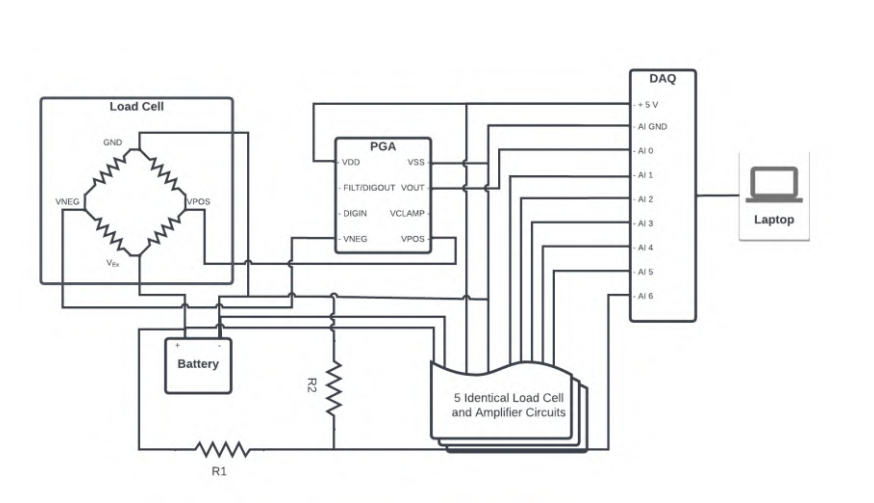
\includegraphics[height=4.5cm]{figures/PrelimSchematic.png}
    \caption{2023 Load string schematic \cite{MFWF_FinalReport2023}}
    \label{fig:LoadStringSchem}
\end{figure}
I constructed the system with one load cell that sends its signal to the input of the AD8556 amplifier, and connected the amplifier output to the borrowed NI USB-6008 DAQ as we did not have the ordered DAQ yet. My first challenge of the semester was just with this initial connection of components. The load cell is essentially just a resistor bridge; the output voltage is half the supply voltage. In this preliminary load string, the suggested voltage to power the load cell was 10 volts, but half of that (5 V) is too close to the amplifiers supply and resulted in no amplified signal. Because of this, I needed to use 5 V to the load cell, which has implications I will discuss in section 2.2.4.
\subsubsection{Unit Test}
\indent With this reduced voltage, I performed a unit test on this preliminary load string setup with gains of 70, 400, 800, and 1280 (maximum for the amplifier used), but only obtained measurable results for the 1280 gain, seen in Figure \ref{fig:Prelim1280}. The LOD (resolution) of this signal is about 30 grams. Assuming that while the lift forces of the flyer will be around the 40 gram mark, this resolution is fine enough to reliably resolve that.
\begin{figure}[htb]
    \centering
    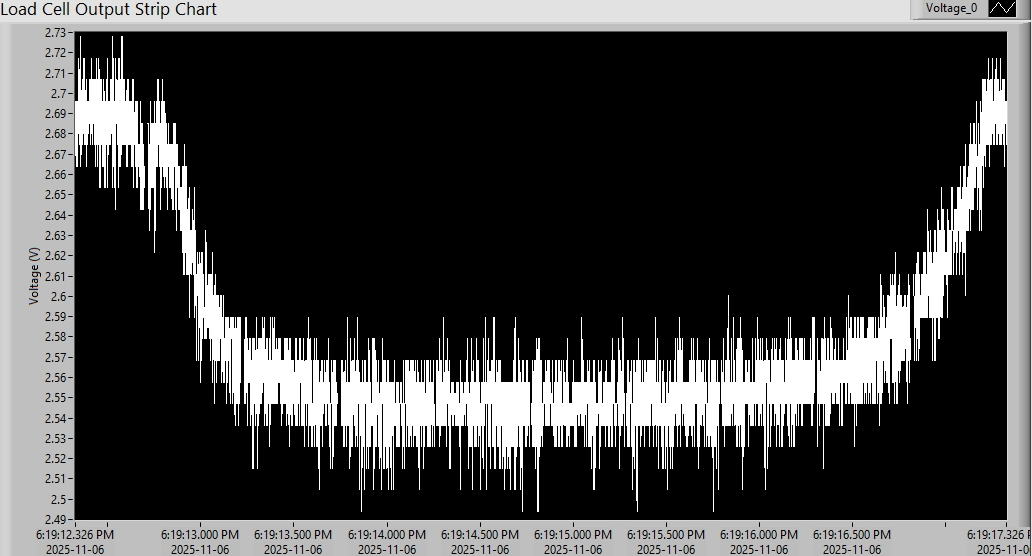
\includegraphics[height=4.5cm]{figures/Prelim1280.png}
    \caption{Preliminary load string unit test results with 1280 gain}
    \label{fig:Prelim1280}
\end{figure}
However, the purpose of the ATP is to also be able to measure any transverse loading produced by the flyer. These forces could be as low as 5 grams and with this setup, that small force would just be lost to noise. A new load string setup was required.
\subsubsection{ATP Test}
With Stan's redesign of the inner frame completed, we tested the load cells on the ATP with static loads in place for the MFWF. Unfortunately, with the tension required to fasten the load cells to the inner frame, the voltage to the DAQ exceeded its limit of +10 volts \cite{NI_USB6008_Specs}. Recall that the load cell and amplifier output a voltage proportional to the gain and applied load. To account for this, the gain was reduced in the amplifier and resulted in a minimum resolution of 200 grams. Unfortunately, this setup wouldn't be able to measure anything the flyer could produce. The load string design needed to be re-visited.
\subsection{Improved Amplifier}
One of the limitations in the preliminary load string was the amplifier. It only supported gains up to 1280 and was limited to an input of 5 volts. Amplifiers can only function if the input signal is less than its supply and recall the load cells output is half the input, meaning this amplifier restricts the load cell to 5 V. The scale of the voltage that is produced by the load cell is directly proportional to it's supply power. That is, at 5 volts, it can produce about 16 mV at its maximum load of 50 newtons (5000 grams). A 10 volt supply doubles this, such that 50 newtons is about 32 mV. What this means is that a higher supply voltage allows a larger range to represent the forces, essentially providing a higher resolution with the same gain.
\subsubsection{Unit Test}
I ordered the AD8421 which has a 32 V maximum supply (well above 5 V), and could apply gain up to 2000 \cite{Analog_AD8421_Datasheet}. Using this, I was able to push the load cell supply to 10 V and performed another unit test. Figure \ref{fig:NewAmpUnitTest} shows the results of the test as the unit load is unloaded. The figure is comparatively more discrete than Figure \ref{fig:Prelim1280}.
\begin{figure}[htb]
\centering
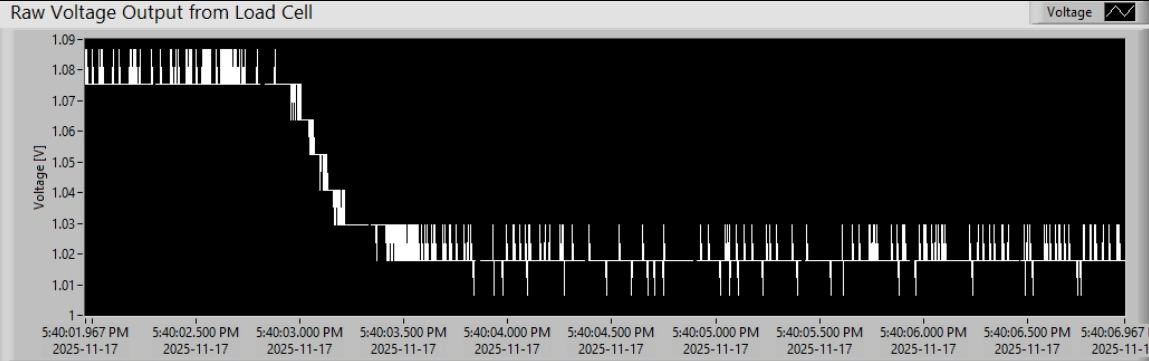
\includegraphics[height=4.5cm]{figures/NewAmpUnitTest.png}
\caption{New amplifier unit test with 2000 gain}
\label{fig:NewAmpUnitTest}
\end{figure}
This was actually due to the limits of the USB-6008 DAQ that was borrowed. It has a 12-bit analog to digital converter (ADC) \cite{NI_USB6008_Specs} which means that the smallest discrete "steps" it can turn an analog signal into is 0.005 V. of 0.01 V. Regardless of this, the test resulted in an LOD of 19 grams; better than the previous setup by about 11 grams, but still not small enough for the ideal of 5 grams.
\subsubsection{ATP Test}
The issue of tension was still present when wanting to test this load string on the ATP. It reached a point where it was thought a new ATP design would be needed to remove the tension in the load cells for a proper reading to be achieved. 
\subsection{Subtracting the Tension}
After discussing the tension problem in one of the weekly presentations, Professor Hashim provided a very insightful suggestion of subtracting the voltage that the tension produces with another known (static) voltage. This allowed the small force produced by the MFWF to be isolated and gained independently of the tension force.

I achieved subtraction by utilizing another AD8421 amplifier. The amplifier is made from op-amp stages that amplify its inputs and subtracts the signals. The first amplifier would take the load cell output and multiply it by some gain such that the output was 10 V plus the small load of the MFWF. I would then use that as an input to the next amplifier and the other input was a clean 10 V, resulting in just the small loads of the flapper as a relatively large voltage. Figure \ref{fig:BBDifference} shows just how many extra components that went in to achieve this subtraction, although most are just for power distribution.
\begin{figure}[htb]
\centering
\begin{subfigure}[t]{.5\textwidth}
  \centering
  \includegraphics[height=4.5cm]{figures/DAQ_BB_Init1.png}
  \caption{Preliminary setup}
  \label{fig:PrelimBB}
\end{subfigure}
\begin{subfigure}[t]{.5\textwidth}
  \centering
  \includegraphics[height=4.5cm]{figures/DAQ_BB_Final1.png}
  \caption{Subtraction setup}
  \label{fig:FinalBB}
\end{subfigure}
\caption{Breadboard setups for (a) preliminary and (b) subtraction load string designs}
\label{fig:BBDifference}
\end{figure}

\subsubsection{Unit Test}
While the new design was modified for testing on the ATP, the USB-6002 DAQ had arrived during the same time period. Instead of a 12-bit ADC, it used a 16-bit ADC \cite{NI_USB6002_Specs}, which allowed finer step sizes to be measured on a signal. To verify this, I performed another unit test with the same setup as in section 2.2.4, but with the new DAQ. Figure \ref{fig:NewDAQUnitTest} shows the measurement of this unit test and compared to Figure \ref{fig:NewAmpUnitTest}, 
\begin{figure}[htb]
    \centering
    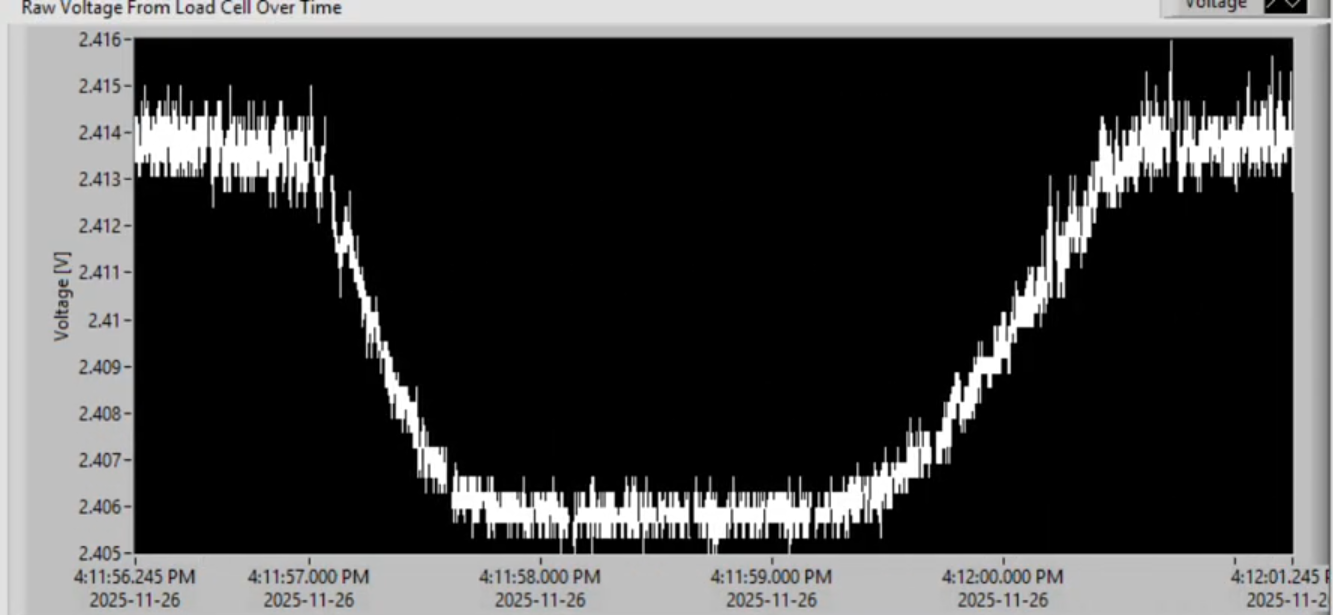
\includegraphics[height=4.5cm]{figures/NewDAQUnitTest.png}
    \caption{USB-6002 DAQ unit test load and unload}
    \label{fig:NewDAQUnitTest}
\end{figure}
it is visually quite an improvement. In fact, the LOD of this test was calculated to be 6.6 grams. Although this resolution is very close to the goal of 5 grams, the load cells themselves have an inaccuracy of 2.5 grams (0.025 N) \cite{Interface_SM_SType}. This means that with the current load cells, we would never be able to measure any force at the scale of the MFWF with 100\% accuracy. Even the thrust could be reported as 50 grams when it is actually 47.5 grams.
\subsubsection{ATP Test}
The ultimate goal of this semester was to commission of the ATP using the hardware we had. Since section 2.2.3 proved that the hardware we had was not adequate, I used the subtraction load string to perform the basis of the commissioning. I fastened a load cell to the top of the ATP and placed different weights on the inner frame to achieve a range of results. The subtraction load string was able to remove the tension while recording the signal. The result was a significant improved measurement of the applied loads. Figures \ref{fig:100gATPLoad} to \ref{fig:10gATPLoad} show the loading or unloading of four different applied loads.
\begin{figure}[htbp]
    \centering
    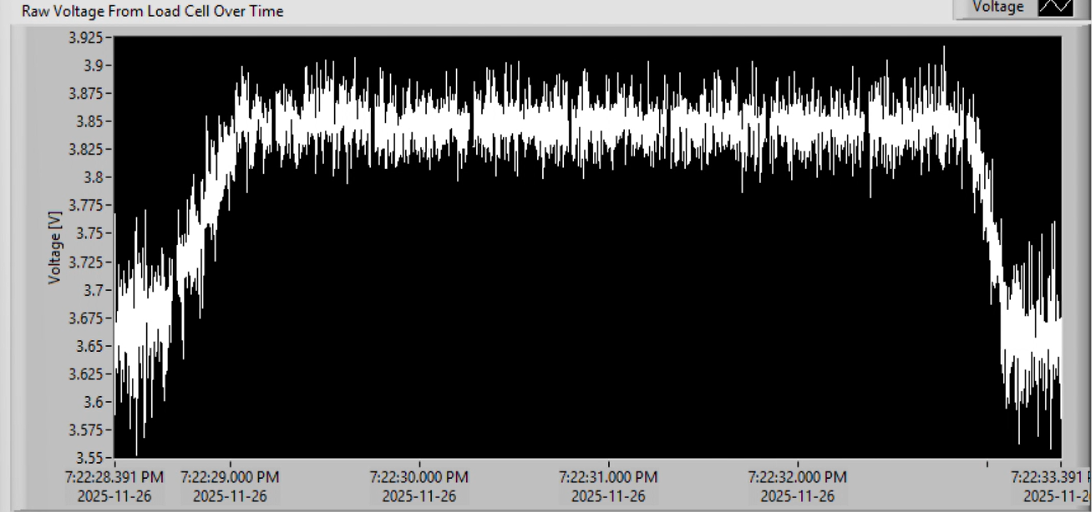
\includegraphics[height=4.5cm]{figures/DoubleAmp_100.png}
    \caption{100-gram ATP test load and unload}
    \label{fig:100gATPLoad}
\end{figure}
\begin{figure}[htbp]
    \centering
    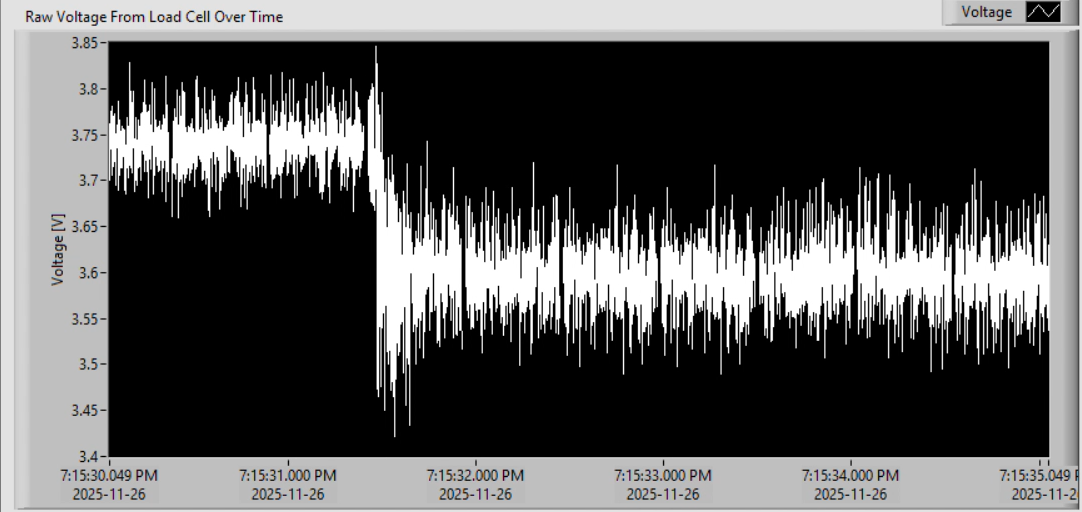
\includegraphics[height=4.5cm]{figures/50g_doubleAmp.png}
    \caption{50-gram ATP test unload}
    \label{fig:50gATPLoad}
\end{figure}
\begin{figure}[htbp]
    \centering
    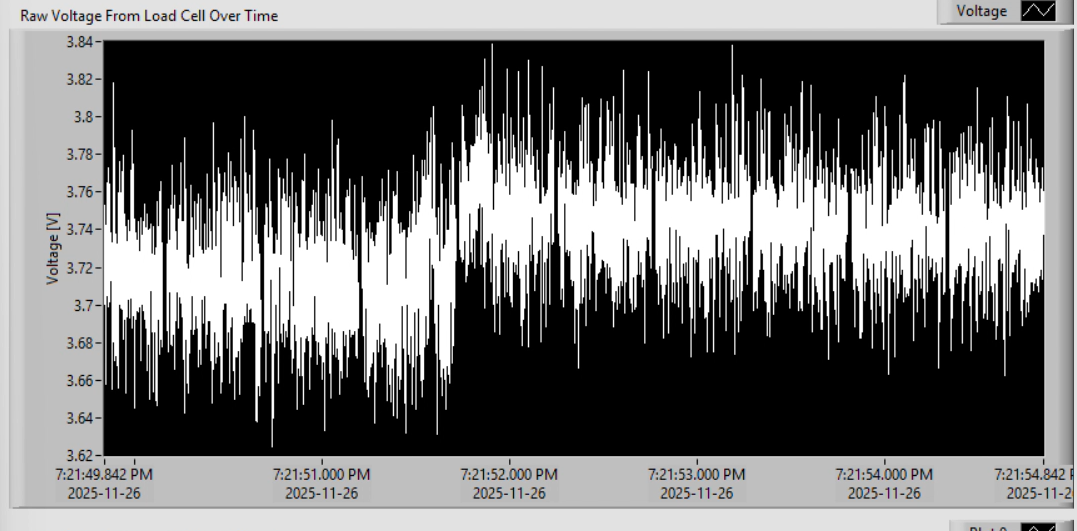
\includegraphics[height=4.5cm]{figures/DoubleAmp_20.png}
    \caption{20-gram ATP test load}
    \label{fig:20gATPLoad}
\end{figure}
\begin{figure}[htbp]
    \centering
    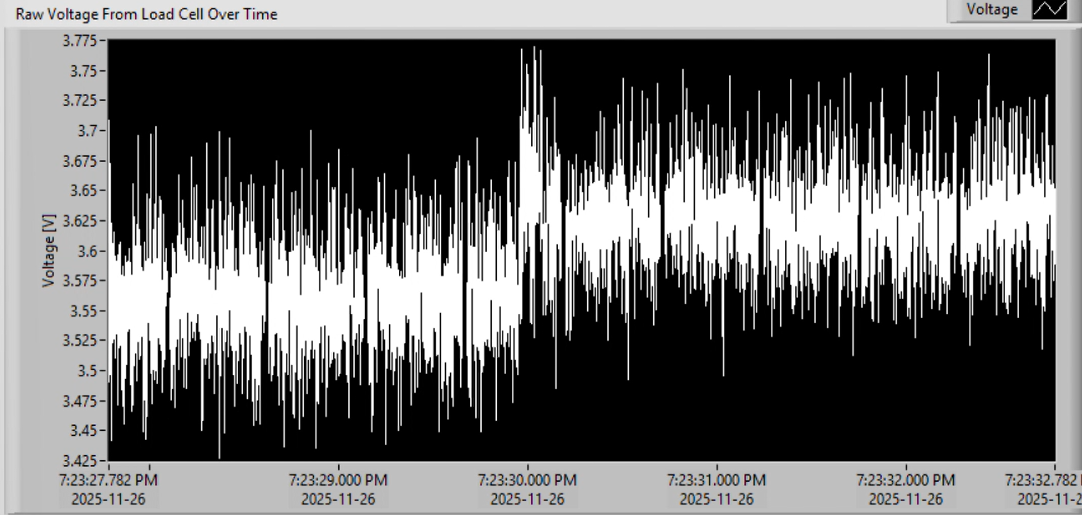
\includegraphics[height=4.5cm]{figures/DoubleAmp_10.png}
    \caption{10-gram ATP test load}
    \label{fig:10gATPLoad}
\end{figure}

Table \ref{tab:ATPTestResultsSummary} shows that the best LOD of the ATP comissioning was 26.6 grams, which represents the 100-gram loading condition. This result is still not as ideal as I'd prefer, but compared to 200 grams, its a large improvement. I do believe that with some tweaking of the load string and some filtering of the signal, it can be viable. An important consideration, however, is the dynamic load of the flapper. With loading and unloading at about 40 Hz frequency, I'm not confident that same resolution can be achieved.

\subsection{Testing Results Summary}
Table \ref{tab:ATPTestResultsSummary} summarizes all the testing that was performed this semester with the different load string designs.
\begin{table} [htbp]
    \centering
    \begin{tabular}{||c|c|c|c||}
        \hline
        Test & $V_{rms}$ Noise $[mV]$ & $S$ [$\frac{mV}{g}$] & $LOD$ [g] \\
        \hline\hline
        Preliminary Unit & 28.3 & 2.8 & 30.3 \\
        \hline
        New Amp. Unit & 7.07 & 1.1 & 19.3 \\
        \hline
        New DAQ Unit & 0.354 & 0.16 & 6.64 \\
        \hline
        ATP Calibration (Best) & 35.4 & 4 & 26.6 \\
        \hline
    \end{tabular}
    \caption{Fall semester ATP test results summary}
    \label{tab:ATPTestResultsSummary}
\end{table}

\subsection{Plan for Winter Semester}
In terms of the signal resolution for a unit load, the load string is capable of determining a load close to the desired 5-gram resolution. However, the load cells inherent accuracy of 2.5 grams limits the fine readings that can be achieved. In terms of ATP comissioning, the subtraction load string is clearly beneficial to remove the tension effects of the current design, but the signals at smaller loads are still quite noisy. The winter semester should have me focusing on improving this signal quality by using some sort of filtering technique.

However, the filtering will have an effect on the dynamic response of the system. While the fine measurements (sub 20 grams) are harder to measure on the ATP, I believe the dynamics of the flyer will have a large impact on the resolution of this signal, and a point should be made to verify a dynamic resolution of even 50 grams if the team is to use this ATP design. The first priority of the winter semester should be to test the ATP with a dynamic load that simulates the flapping of the MFWF. With the results of this test, and some tuning of the subtraction load string, I indent to have a reasonable understanding of how the ATP will perform with the MFWF mounted. Given that professor Hashim has been influential to this side of the ATP team, I will be using him as a resource to gain more knowledge of how the fine resolution of a dynamic flyer can be achieved. Ultimately, my goal before the winter semester ends is to have an exhausted testing report of this ATP design to prove its viability for the MFWF team to use during their flight tests. 